\chapter{BADAM: A Public Dataset for Baseline Detection in Arabic-script Manuscripts}
\chaptermark{Baseline Detection in Arabic Manuscripts}
\label{ch:hip}
\thispagestyle{empty}
\vfill
This chapter has been published as \fullcite{kiessling2019badam}

\newpage
\section*{Abstract}
	The application of handwritten text recognition to historical works is
	highly dependant on accurate text line retrieval. A number of systems
	utilizing a robust baseline detection paradigm have emerged recently
	but the advancement of layout analysis methods for challenging scripts
	is held back by the lack of well-established datasets including works
	in non-Latin scripts. We present a dataset of 400 annotated document
	images from different domains and time periods. A short elaboration on
	the particular challenges posed by handwriting in Arabic script for
	layout analysis and subsequent processing steps is given.  Lastly, we
	propose a method based on a fully convolutional encoder-decoder network
	to extract arbitrarily shaped text line images from manuscripts.

\section{Introduction}

Layout analysis as a major preprocessing step for text recognition is currently
considered the limiting factor in the digitization of historical documents both
handwritten and printed, especially so for non-Latin writing systems such as
Arabic. With the rise of Digital Humanities and large scale institutional
digitization projects a significant community of researchers engaged in the
improvement of layout analysis on historical material has formed.

The most visible expression of this is a long-standing series of competitions
evaluating either layout analysis in isolation
\cite{gatos2011icdar2009,antonacopoulos2009icdar,gatos2010icfhr,antonacopoulos2011historical,antonacopoulos2013icdar,murdock2015icdar,diem2017cbad}
or as part of a larger text recognition task such as
\cite{antonacopoulos2015icdar2015}. Unfortunately, these competitions concern
themselves almost exclusively with Western texts written in Latin script
despite some efforts to organize competitions on material that is
insufficiently treated by current methods.

This euro- and anglocentric focus in document analysis research has changed to
some extent recently. Although not directly connected to layout analysis
\cite{burie2016icfhr} presented binarization, keyword spotting, and isolated
character recognition challenges on Balinese palm leaf manuscripts.
\cite{clausner2018icfhr} included a layout analysis task on Arabic manuscripts
but notably lacked a publicly available training dataset, except 15
representative images for informational purposes, and participation remained
rather modest.

Recognizing that there is an obvious need for a large dataset of non-Western
texts we propose a dataset based on one of the most geographically and
chronologically extensive manuscript cultures, the Arabic and Persian one. This
choice is motivated by multiple reasons: the exceptional size of the available
material covering a wide range of topics and styles, complexity of layout
rarely encountered in Latin manuscripts, and a large community of scholars
working on Arabic-script manuscripts.

In addition, we strive to provide a dataset sufficient in size to support
development of state-of-the-art machine learning ap\-proach\-es to layout analysis
which despite increasing popularity for Latin documents
\cite{barakat2018text,quiros2018multi,fink2018baseline} has seen limited uptake
for other writing systems.

\subsection{Related work}

Existing layout analysis datasets capture text lines in a variety of data
models. These range from polygons
\cite{fischer2011transcription,simistira2016diva,clausner2018icfhr}, to
sub-word bounding boxes \cite{kassis2017vml}, down to explicit pixel labeling
\cite{gatos2010icfhr}. Some others such as
\cite{antonacopoulos2015icdar2015,antonacopoulos2011historical} also include
extensive metadata such as reading order, text order, or full transcriptions.

A new paradigm reducing text line segmentation to the successful detection of a
continuous sequence of line segments has been established by the ICDAR 2017
Competition on Baseline Detection \cite{diem2017cbad}. There are a plethora of
benefits to this minimalistic model: better expression of highly curved
baselines in comparison to bounding boxes, lower complexity of training data
production than full polygons, easier modelling by semantic segmentation models
because of object separability, and the existence of an evaluation scheme
\cite{gruning2018read} that is more directly linked to real world recognition
error rates than raw pixel accuracy.

\begin{figure}[h]
	\centering
	\begin{subfigure}{.9\columnwidth}
		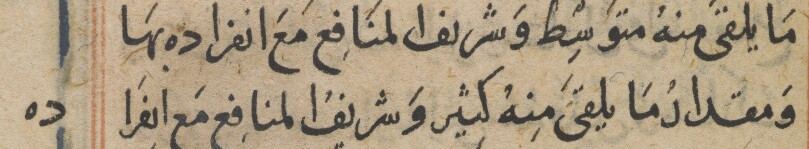
\includegraphics[width=\textwidth]{or9452_margin.jpg}
		\caption{Expulsion of text into the margin}
		\label{fig:margin}
	\end{subfigure}
	\vskip\baselineskip

	\begin{subfigure}{.9\columnwidth}
		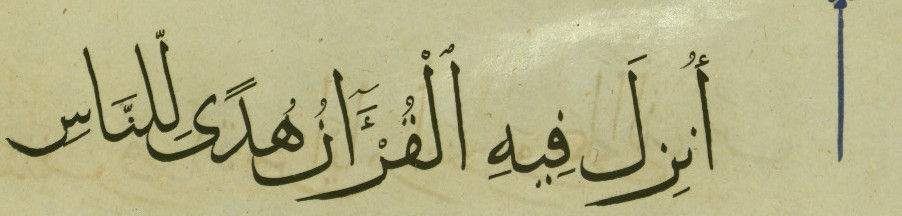
\includegraphics[width=\textwidth]{w561_slanted.jpg}
		\caption{Per-word slanted baselines}
		\label{fig:slanted}
	\end{subfigure}
	\vskip\baselineskip

	\begin{subfigure}{.9\columnwidth}
		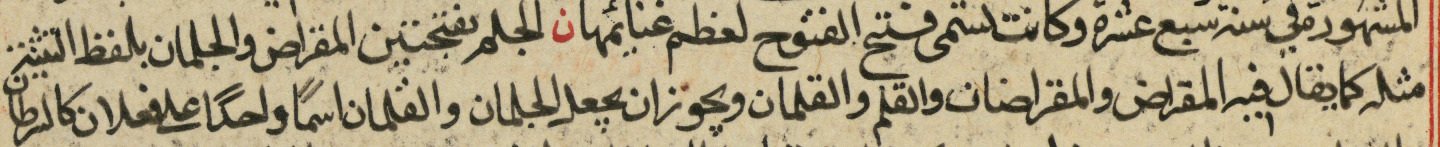
\includegraphics[width=\textwidth]{w590_heaping.jpg}
		\caption{Heaping of words at end of line}
		\label{fig:heaping}
	\end{subfigure}
	\vskip\baselineskip

	\begin{subfigure}{.9\columnwidth}
		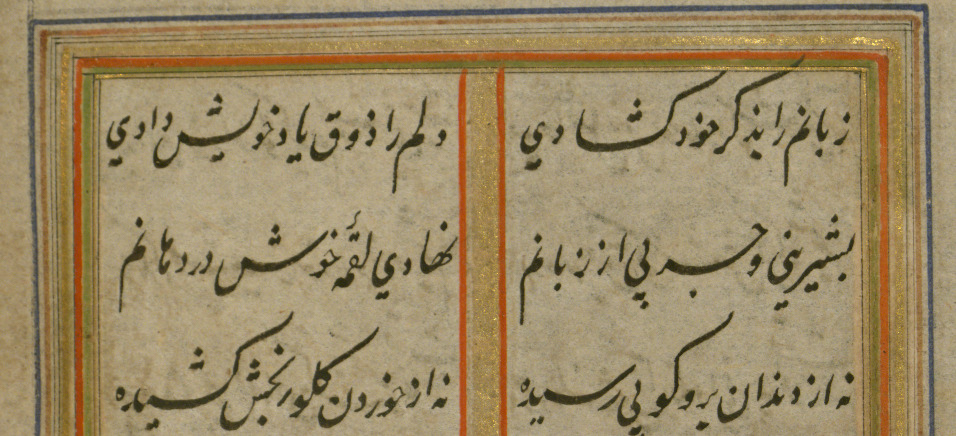
\includegraphics[width=\textwidth]{w644_poetry.jpg}
		\caption{Pseudo-columns in Persian poetry}
		\label{fig:poetry}
	\end{subfigure}
	\caption{Aspects of Arabic-script handwriting}
\end{figure}

\begin{figure}[h]
	\centering
	\begin{subfigure}{.9\columnwidth}
		
\includegraphics[width=\textwidth]{img792_expulsion_anno.jpg}
		\caption{Annotation of dislocated fragments in margin}
		\label{fig:anno_margin}
	\end{subfigure}
	\vskip\baselineskip

	\begin{subfigure}{.9\columnwidth}
		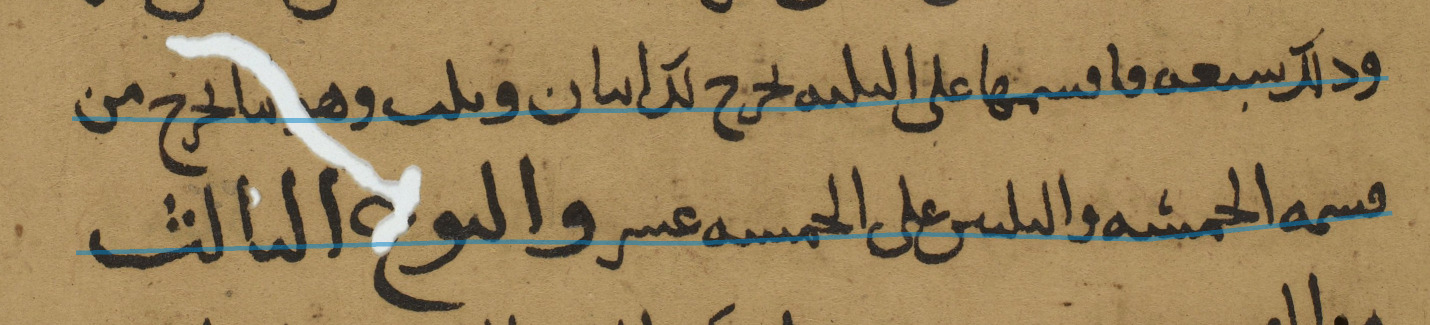
\includegraphics[width=\textwidth]{ljs293_holes_anno.jpg}
		\caption{Holes in writing surface}
		\label{fig:anno_holes}
	\end{subfigure}
	\vskip\baselineskip

	\begin{subfigure}{.9\columnwidth}
		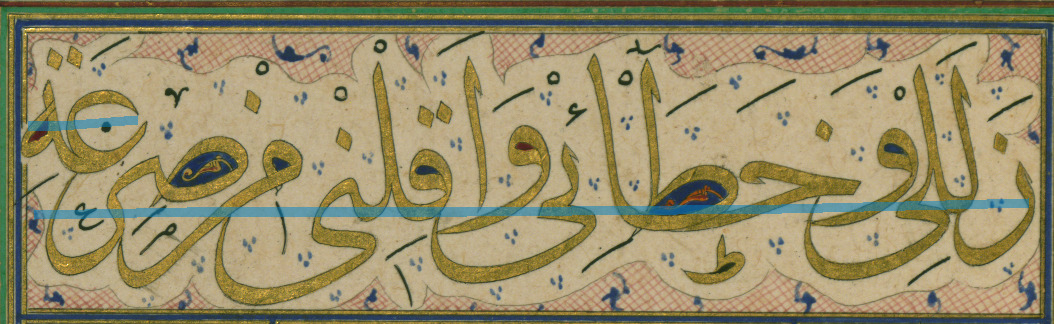
\includegraphics[width=\textwidth]{w579_pwb_anno.jpg}
		\caption{Per-word baseline annotation through imaginary baseline}
		\label{fig:anno_pwb}
	\end{subfigure}
	\vskip\baselineskip

	\begin{subfigure}{.9\columnwidth}
		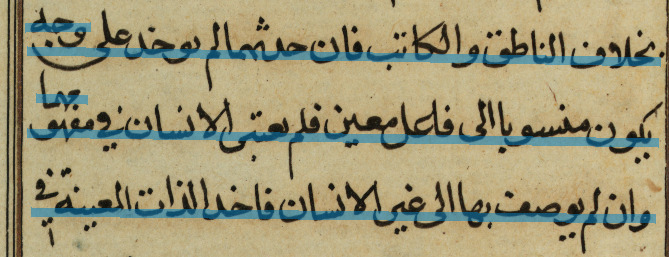
\includegraphics[width=\textwidth]{w591_stacking_anno.jpg}
		\caption{Separate annotation of heaped elements with complete overlap vs single baseline for partial overlap}
		\label{fig:anno_stacking}
	\end{subfigure}
	\vskip\baselineskip

	\begin{subfigure}{.9\columnwidth}
		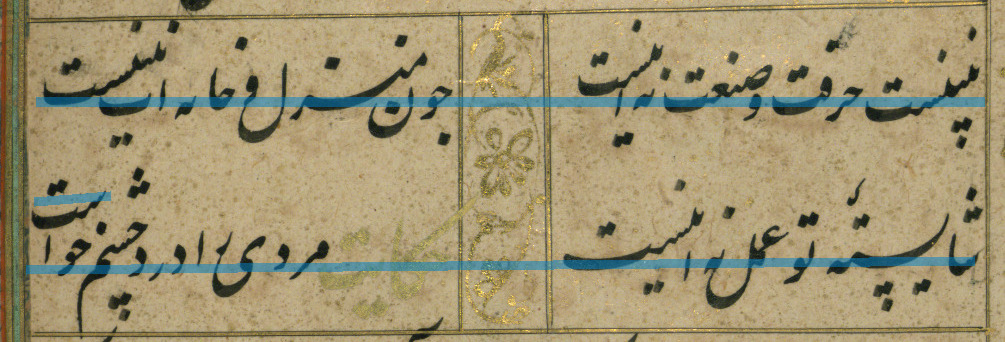
\includegraphics[width=\textwidth]{w619_poetry_anno.jpg}
		\caption{Joint annotation of half-verses as a single baseline}
		\label{fig:anno_poetry}
	\end{subfigure}
	\vskip\baselineskip

	\begin{subfigure}{.9\columnwidth}
		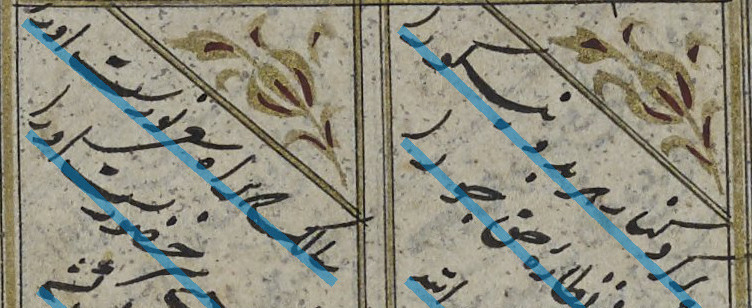
\includegraphics[width=\textwidth]{ljs44_slp_anno.jpg}
		\caption{Separated annotation of slanted half-verses}
		\label{fig:anno_slp}
	\end{subfigure}

	\caption{Examples of annotation guideline application (baseline indicated with opaque blue polyline)}
\end{figure}

\section{Dataset}

\begin{figure*}[ht]
	\centering
	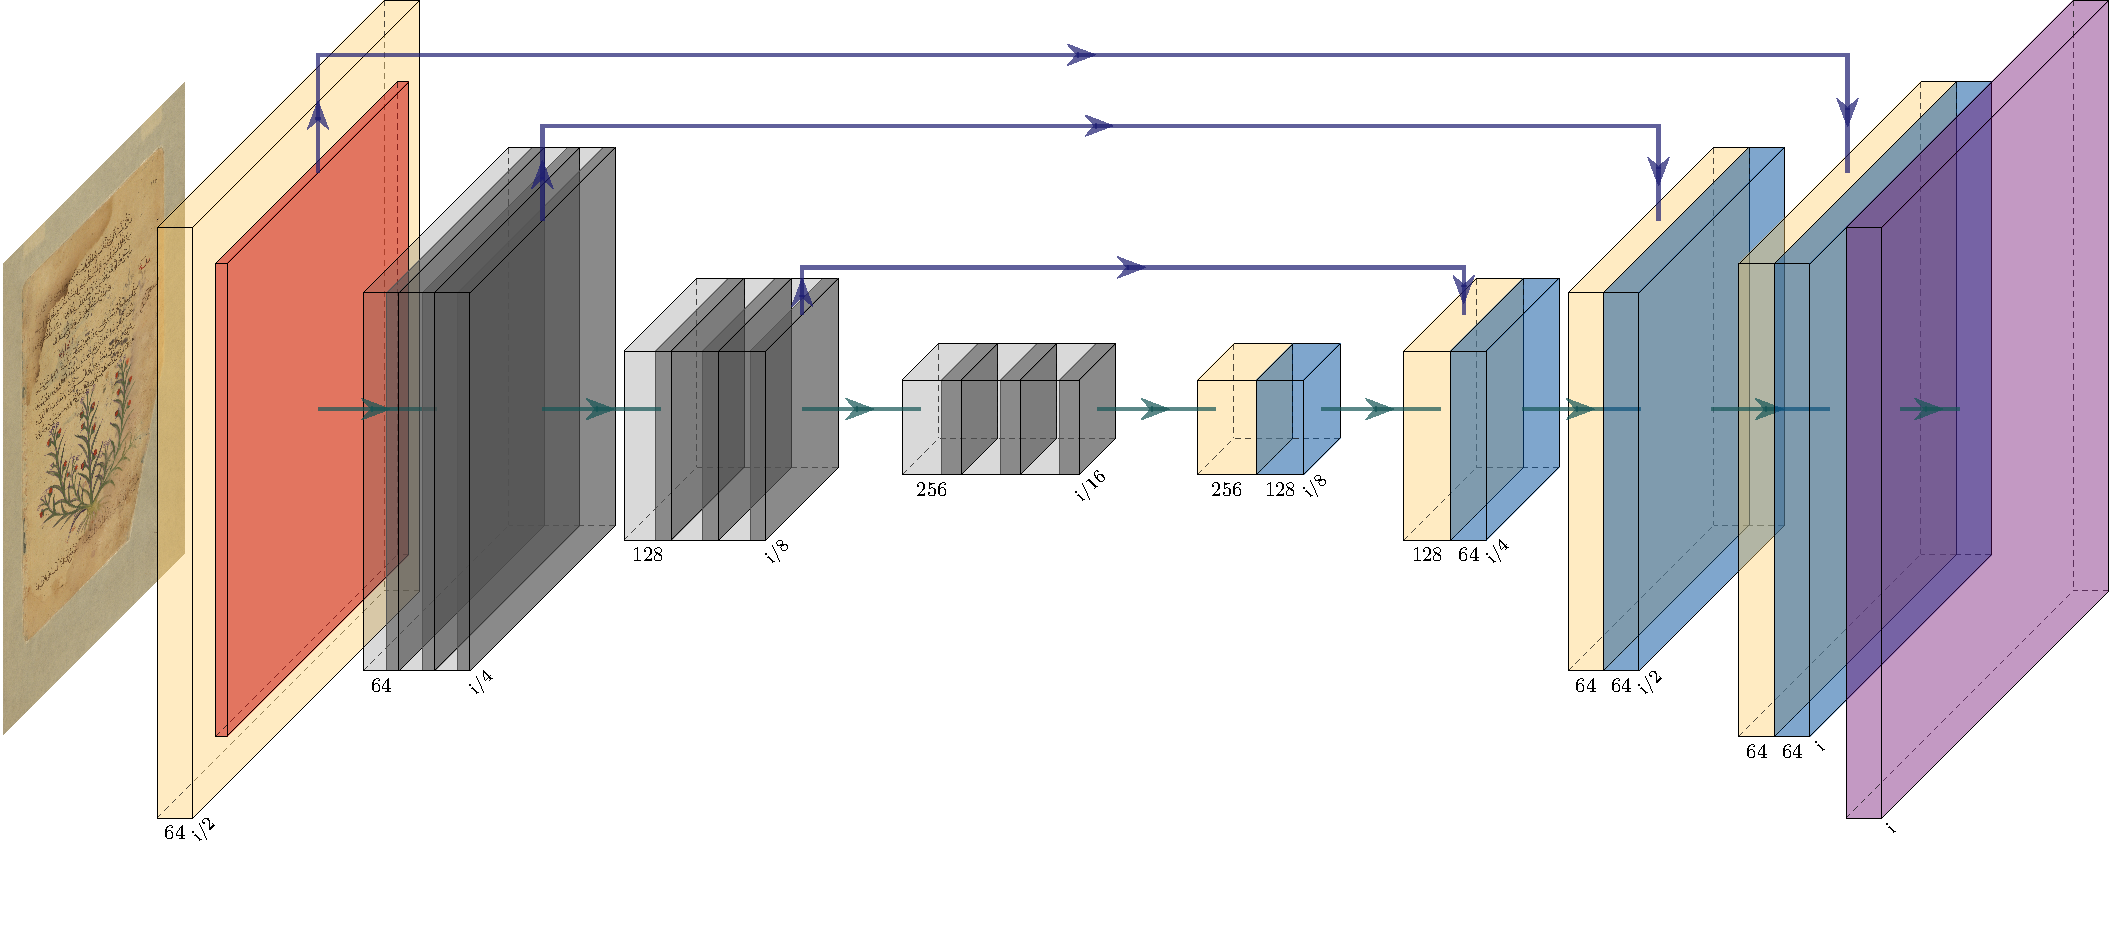
\includegraphics[width=\textwidth]{diag}
	\caption{Architecture of the baseline labelling network. Dropout and
	batch/group normalization layers are omitted. (beige: convolutional layers +
	ReLU, red: max pooling, grey: ResNet blocks, blue: transposed
	convolutions, purple: convolution + sigmoid)}
	\label{fig:resunet}
\end{figure*}

The publicly available and freely licensed BADAM dataset contains 400 annotated
scanned page images samples from four digital collections of Arabic and Persian
language manuscripts.

\subsection{Baselines and Arabic Typography}

A term arising chiefly from Western typography, the baseline is defined as the
virtual line upon which most characters rest with descenders extending below.

While many Arabic handwritten texts present only a single baseline per logical
text line a large number of documents, especially calligraphic works in Thuluth
and Nastaliq style, display per word slanted baselines (Fig.
\ref{fig:slanted}), multiple baseline levels, and dislocation of fragments into
the margins or above other text in the line (heaping) (Fig. \ref{fig:heaping}
and \ref{fig:margin}). Most of these cases fulfill the purpose of text
justification as hyphenation has been considered unacceptable in Arabic writing
for the vast majority of the script's use.

As an additional complication, verses in Arabic poetry almost exclusively
consist of two hemistichs, with the half-verse break forming pseudo-columns as
shown in Fig. \ref{fig:poetry}. In some cases there is a combination of
pseudo-columns and true multi-column text.

We therefore adopt a modified baseline definition that is oriented towards the
current capabilities of text line recognition and reading order determination
systems. Text lines are annotated with a single baseline extended through the
majority of the line text, except in the cases of majority-overlap heaping
(Fig. \ref{fig:anno_stacking}) and dislocation into the margin (Fig. \ref{fig:anno_margin}).
In the case of slanted per-word baselines without horizontal overlap a baseline
is drawn through an imaginary rotation point at each word (Fig. \ref{fig:anno_pwb}). A
baseline is split in multi-column text and at marginalia/main body boundaires.
The hemistichs of poems are annotated as a single baseline per verse
(Fig. \ref{fig:anno_poetry}), except in the case of 45 degree slanted half-verses
(Fig. \ref{fig:anno_slp}) that cannot easily be connected. In fragmentary material the
baseline is continued through faded ink and split at holes in the writing
surface (Fig. \ref{fig:anno_holes}).

These annotation guidelines amount to a conservative estimation of the
capabilities of layout analysis systems, specifically their capacity to
associate disconnected elements on the page belonging to the same logical line.
It is relatively easy to extend the dataset with a more abstract data model
that groups multiple baselines into a logical text line and we expect to do so
in the future.


\subsection{Data}


42 manuscripts were randomly sampled from the collections of the Qatar Digital
Library (15), the digital collection of the Walters Art Museum (13), the
Beinecke Rare Book and Manuscript Library (6), and University of Pennsylvania
Libraries manuscript collection (8). 10 single page images chosen were
annotated for each manuscript with the
labelme\footnote{https://github.com/wkentaro/labelme} image annotation tool
with the exception of 4 shorter manuscripts from the Beinecke Library
containing only 3 to 7 pages. Pages were selected manually for being
representative of each work. Overall, there are 10770 lines in the corpus with
a range of 3 to 176 lines per manuscript page ($\mu = 30.3, \sigma = 22.1$).
The majority of the corpus is written in the Naskh style with the remainder
being split between Thuluth, Nastaliq, and Kufic. Other regional styles such as
ones used in Ottoman writing are currently absent.

A variety of writings is represented in the corpus:

\begin{enumerate}
	\item Medical treatises including poetry with extensive marginalia
	\item Works on logic, commentary on astronomy and arithmetic
	\item Illuminated prayer books and religious texts
	\item Texts on law such as legal glossaries
	\item Illuminated poetic works in Persian and Arabic
	\item Treatises on the legality and rules of chess including extensive diagrams and marginalia
\end{enumerate}

The scan quality of the material varies according to the collection it was
sourced from. While all are produced to a professional standard, the resolution
varies considerably from 200dpi in the QDL, to 300 dpi in material from the
Walters and Beinecke, and 500dpi at the University of Pennsylvania.

A predefined random split into a 320 page training set and a 80 page test set
is provided. The annotation is available in both PAGE XML and bit mask image
formats.  The corpus including both sampled images and ground truth is publicly
released under CC-BY-SA 2.0 and available for download on the 
Zenodo\footnote{\url{https://doi.org/10.5281/zenodo.3274428}} research data archive.

\begin{figure}[]
	\begin{subfigure}[b]{.475\columnwidth}
		\centering
		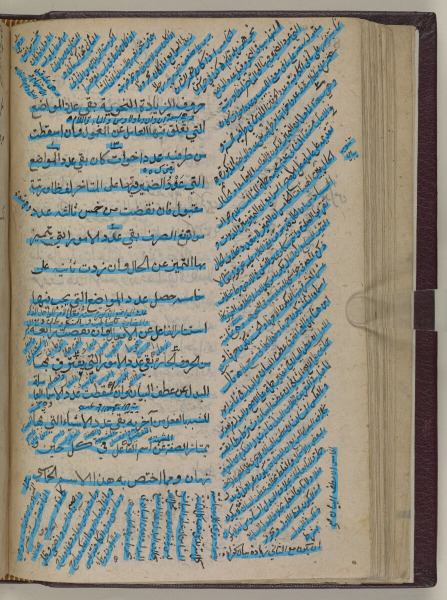
\includegraphics[width=\textwidth]{curved.jpg}
	\end{subfigure}
	\hfill
	\begin{subfigure}[b]{.475\columnwidth}
		\centering
		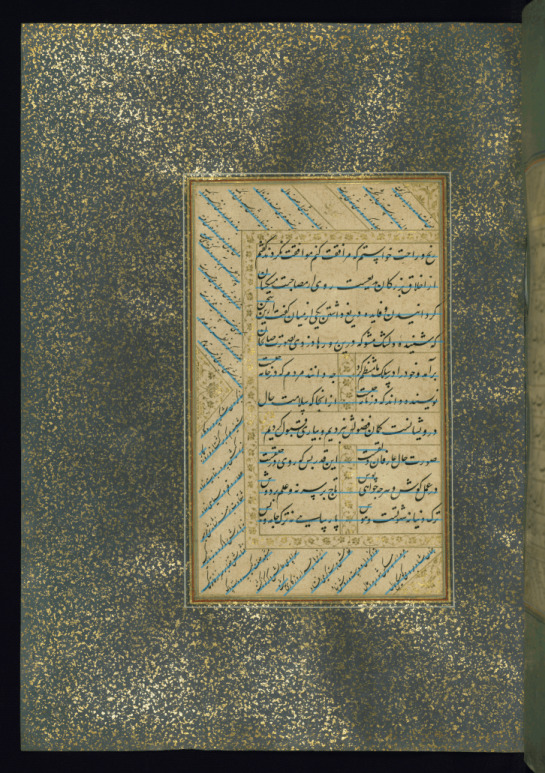
\includegraphics[width=\textwidth]{poetry.jpg}
	\end{subfigure}
	\vskip\baselineskip
	\begin{subfigure}[b]{.475\columnwidth}
		\centering
		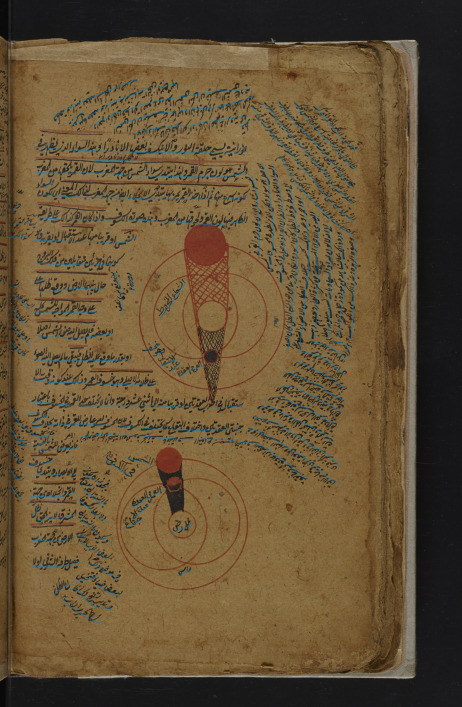
\includegraphics[width=\textwidth]{diagrams.jpg}
	\end{subfigure}
	\hfill
	\begin{subfigure}[b]{.475\columnwidth}
		\centering
		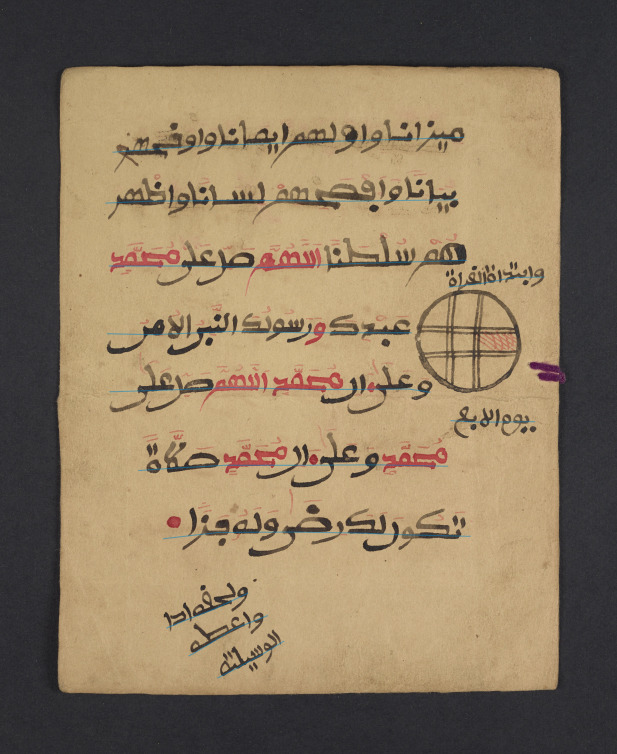
\includegraphics[width=\textwidth]{kufic.jpg}
	\end{subfigure}
	\caption{4 sample pages from the corpus}
	\label{fig:samples}
\end{figure}

\begin{figure}[ht!]
	\centering
	\begin{subfigure}[t]{.475\columnwidth}
		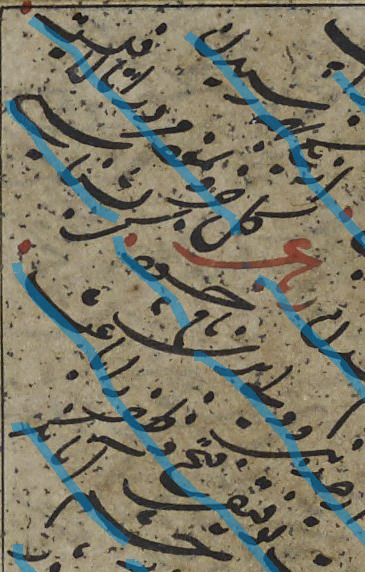
\includegraphics[width=\textwidth]{fail_calli.jpg}
		\caption{Splitting of calligraphic writing in third/fourth line from top.}
		\label{fig:calli}
	\end{subfigure}
	\hfill
	\begin{subfigure}[t]{.475\columnwidth}
		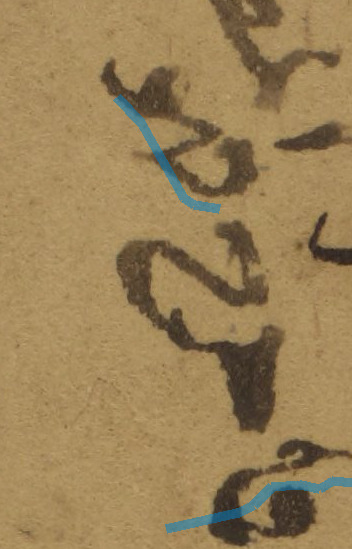
\includegraphics[width=\textwidth]{fail_vert.jpg}
		\caption{Misrecognition of vertical text}
		\label{fig:vert}
	\end{subfigure}
	\begin{subfigure}[b]{\columnwidth}
		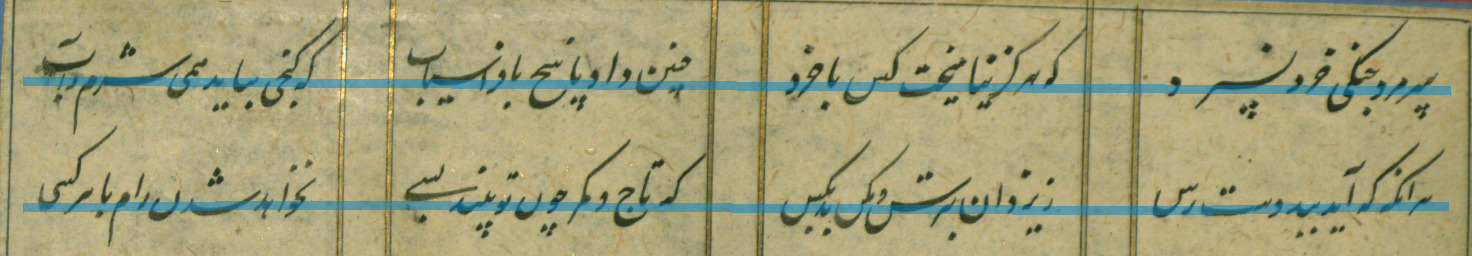
\includegraphics[width=\textwidth]{fail_4col.jpg}
		\caption{Incorrect splitting of logical 2-column poetry}
		\label{fig:4col}
	\end{subfigure}
	\begin{subfigure}[b]{\columnwidth}
		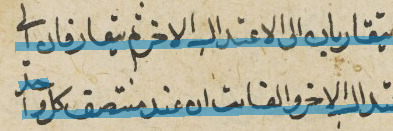
\includegraphics[width=\textwidth]{fail_heap.jpg}
		\caption{Missed heaped letter in top line, correct example on the bottom}
		\label{fig:misheap}
	\end{subfigure}
	\caption{Common error modes of the LA system}
\end{figure}

\section{Baseline Method}

Our method consists of two main stages: a pixel level classification of
baselines followed by a lightweight baseline extraction step. We call this
approach convolutional baseline layout analysis (C-BLLA).

In the first stage a fully convolutional encoder-decoder neural network is used
to assign each pixel to a either background or baseline. The second stage is a
script- and layout-agnostic postprocessing step operating on the heatmap
produced by the neural network. Baselines are vectorized into polylines which
are then used to extract rectified rectangular line image suitable for
processing by an HTR line recognition system.

\subsection{Pixel Labeling}

The dense pixel-labelling of baselines is performed with a modified U-Net
architecture \cite{ronneberger2015u}. U-Nets and similar fully convolutional
networks \cite{long2015fully} are state-of-the-art for general semantic
segmentation tasks and have achieved excellent results on the cBAD dataset
\cite{diem2017cbad}.

The backbone model consists of the first 3 blocks of a 34-layer ResNet in the
contracting path followed by 4 3$\times$3 convolution-transposed convolution
blocks in the expanding paths with group normalization
\cite{DBLP:journals/corr/abs-1803-08494} ($G = 32$) and dropout ($p = 0.1$)
employed after each layer and block respectively. A final 1$\times$1
convolutional layer reduces the dimensionality of the input-sized 64-channel
feature map to 1, followed by a sigmoid activation. An overall diagram of the
network is shown in Fig. \ref{fig:resunet}.

In order to improve generalization, the contracting path is pretrained on
ImageNet classification and kept fixed during training of the upsampling
blocks. Trainable layers are initialized using the He scheme
\cite{he2015delving}. We use the Adam optimizer with moderate weight decay
($\alpha = 10^{-4}, \beta_1 = 0.9, \beta_2 = 0.999, w = 10^{-6}$) and early
stopping on the binarized F1 score of the validation set.  The network is
trained on whole color images with the inputs being scaled to a size of 1200
pixels on the shortest edge to limit memory usage.


\subsection{Baseline Estimation}

The final sigmoid activation map has to be binarized prior to baseline
vectorization. To suppress noise resulting in a higher number of skeleton
branches causing a slow down of end point calculation in the next step, the raw
heatmap is smoothed with a gaussian filter ($\sigma = 1.5$) first, followed by
binarization with hysteresis thresholding ($t_{low} = 0.3, t_{high} = 0.5$)

The binarized image is then skeletonized \cite{lee1994building} and 1-connected
end point candidates are extracted with a discrete convolution. As the skeleton
often contains small branches, determining the actual end points of the
centerline skeleton can be challenging. We treat all points along the skeleton
as nodes in a graph and assume the true end points are the ones furthest apart
on the skeleton. The actual baseline is thus the path of the maximum graph
diameter of all possible candidate combinations. This path is then vectorized
into a polyline with the Douglas-Peucker algorithm
\cite{douglas1973algorithms}.

\subsection{Line extraction}

Vectorized baselines have to be converted into rectangular line images for
classification by HTR recognition systems. Given that the baselines found by
the system can be highly curved, even circular or spiral-formed, each polyline
should be rectified by projecting its line segments and their respective
environment consecutively onto a straight baseline.

For each line segment we compute an orthogonal vector of appropriate length
including the desired area around the baseline determining the control points
above and below the segment at each step. The rasterizations produced by
Bresenham's line between both control points at each step are then appended to
the rectified line.

According to the results reported in \cite{romero2015influence} and our own
verification on a typeset synthetic dataset the size of the environment
extracted around the baseline is not crucial to recognition accuracy as long as
the line contents are contained in the rectified line image. We estimate the
per-line environment by thresholding the input image with
\cite{sauvola2000adaptive}, calculating connected components under each
baseline, and finding the maximum orthogonal distances of their edges above and
below the baseline.


\section{Evaluation}

We evaluated the proposed method on the 80 page test set using the method
described in \cite{gruning2018read}. The results are shown in table
\ref{tab:foo}. The metrics are slightly lower for our dataset than on the Latin
cBAD dataset with a large gap in recall caused by a failure to extract heaped
fragments (Fig. \ref{fig:misheap}) and vertical writing (Fig. 
\ref{fig:vert}). On the other hand many missegmented lines are ornate or
slanted (Fig. \ref{fig:calli}), poetry (Fig. \ref{fig:4col}) indicating
that the network has not been able to learn a coherent model for these features
on the dataset.

\begin{figure}[ht!]
	\centering
	\begin{subfigure}[t]{\columnwidth}
		
\includegraphics[width=\textwidth]{cor_color.jpg}
		\caption{Detection of lines containing differently colored keywords}
		\label{fig:cor_color}
	\end{subfigure}
	\begin{subfigure}[t]{\columnwidth}
		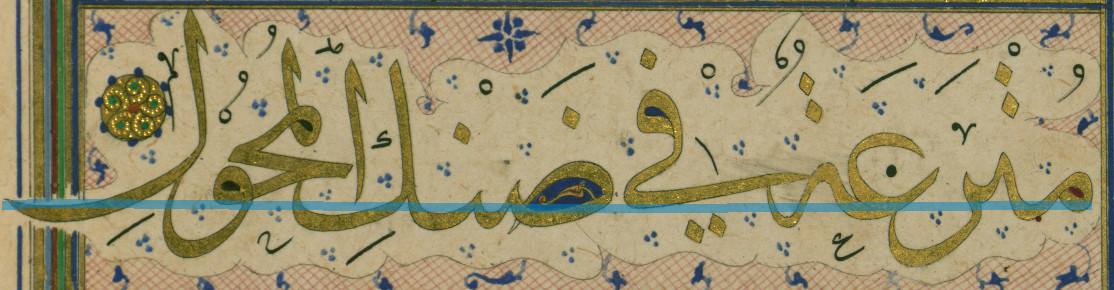
\includegraphics[width=\textwidth]{cor_color_gold.jpg}
		\caption{Detection of lines illuminated in gold}
		\label{fig:cor_color_gold}
	\end{subfigure}
	\begin{subfigure}[b]{\columnwidth}
		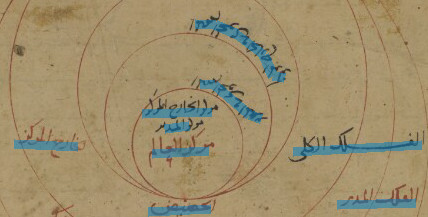
\includegraphics[width=\textwidth]{cor_diagram.jpg}
		\caption{Extraction of labels in a diagram}
		\label{fig:cor_labels}
	\end{subfigure}
	\caption{Strengths of the C-BLLA method}
\end{figure}

Apart from the higher flexibility of the baseline paradigm in comparison to
older text line modelling approaches, C-BLLA has a number of other strengths.
The method is largely robust against changes in text coloration such as red
keywords (Fig. \ref{fig:cor_color_gold}) or lines illuminated in gold (Fig.
\ref{fig:cor_color_gold}) without the need for binarization of input images.
Further it is able to ignore both border elements (support platforms, scales,
and holding clips) and illustrations without an explicit text content
extraction step. As illustration are processed jointly, textual labels can be
detected albeit as a unstructured collection of lines (Fig.
\ref{fig:cor_labels}).

There are some limitations to semantic segmentation in the context of layout
analysis. These methods are inherently incapable of extracting overlapping and
crossing text lines. This is exacerbated by the downsampling performed before
inference which can cause inadvertent line merging in documents with closely
written interlinear notes or commentary directly adjacent to main text. 

The overall agreement in accuracy between the different datasets indicates that
modern semantic segmentation methods can be employed for a wide variety of
scripts when coupled with appropriate script-agnostic postprocessing. It
remains to be seen if the accuracy gap between both datasets can be closed with
general purpose systems that are not optimized for a particular set or if
script-specific adaptations, such as specialized postprocessing, will be
necessary.

\begin{table}[htbp]
\begin{center}
\caption{Results for the cBAD 2017 dataset and BADAM}
\label{tab:foo}
\begin{tabularx}{\columnwidth}{lXXX} \toprule
& \textbf{P-val} & \textbf{R-val} & \textbf{F-val}\\
\addlinespace
\textbf{cBAD Simple Track}\ \\ \midrule
BYU & 0.878 & 0.907 & 0.892\\
dhSegment & 0.943 & 0.939 & 0.941\\
ARU-Net & 0.977 & 0.980 & 0.978 \\
C-BLLA & 0.944 & 0.966 & 0.954\\
\addlinespace
\textbf{BADAM}\ \\ \midrule
C-BLLA & 0.941 & 0.901 & 0.924\\
\bottomrule
\end{tabularx}
\end{center}
\end{table}

\section{Conclusion}

We presented a new dataset consisting of 400 annotated page scans of Arabic and
Persian manuscripts spanning a wide range of topics and dates of production.
Documents in the dataset present various degradations and large differences in
the complexity of layout and writing styles. Many of the difficulties posed by
them are specific to the Arabic script and should challenge the generalization
power of even up-to-date layout analysis methods optimized for Latin script
historical documents. While acknowledging that the annotation guidelines
oriented on capabilities of current recognition algorithms will likely evolve
in the future, our work contributes a solid foundation for comparable
evaluation for document analysis researchers.

In addition we describe a baseline system for line extraction from the corpus
and evaluate its results, showing that even state-of-the-art methods have
difficulties segmenting challenging Arabic handwriting as accurately as
Latin manuscripts.
